\section{Auswertung}
\label{sec:Auswertung}

\subsection{Eichung des Magnetfeldes}
\label{sec:Magnetfeld}
Zu Beginn des Versuchs muss das Magnetfeld, durch das später die Aufspaltung der Energieniveaus hervorgerufen wird, geeicht werden. 
Dafür wird mit hilfe einer Hall-Sonde die Magnetfeldstärke $\vec{B}$ des verwendeten Elektromagneten, in Abhängigkeit von dem 
angeschlossenen Strom $I$ bestimmt.
Die Messwerte sind in Tabelle \ref{tab:Magnetfeld} aufgelistet.
In Abbildung \ref{fig:Magnetfeld} sind die Messwerte zusammen mit einer Ausgleichskurve der Form,

\begin{equation}
  f(x) = a x^2 + b x + c ,
\end{equation}
  eingetragen.
  Die Parameter, zur Berechnung der genutzten Magnetfeldstärke, lauten: \\
  $a = -5,70 \pm 0,27$ mT \\
  $b = 119,03 \pm 2,27$ mT \\
  $c = -5,25 \pm 3,92$ mT \\
 

\begin{table}
  \centering
  \footnotesize
  \caption{Gemessenes Magnetfeld in Abhängigkeit von der Stromstärke.}
  \label{tab:Magnetfeld}

  \begin{tabular}{r r | r r}
    \toprule
    I [A] & B [mT] & I [A] & B [mT] \\
    \midrule
    0   & 7,6   & 4,5   & 418,7 \\
    0,5 & 54,2  & 5     & 454,3 \\
    1   & 102,5 & 5,5   & 482,1 \\
    1,5 & 151,6 & 6     & 509,1 \\
    2   & 203,1 & 6,5   & 530   \\
    2,5 & 255,1 & 7     & 547,8 \\
    3   & 297,4 & 7,5   & 563,3 \\
    3,5 & 338,3 & 8     & 577,5 \\
    4   & 381,9 & & \\
    \bottomrule
  \end{tabular}
\end{table}

\begin{figure}[H]
  \centering
  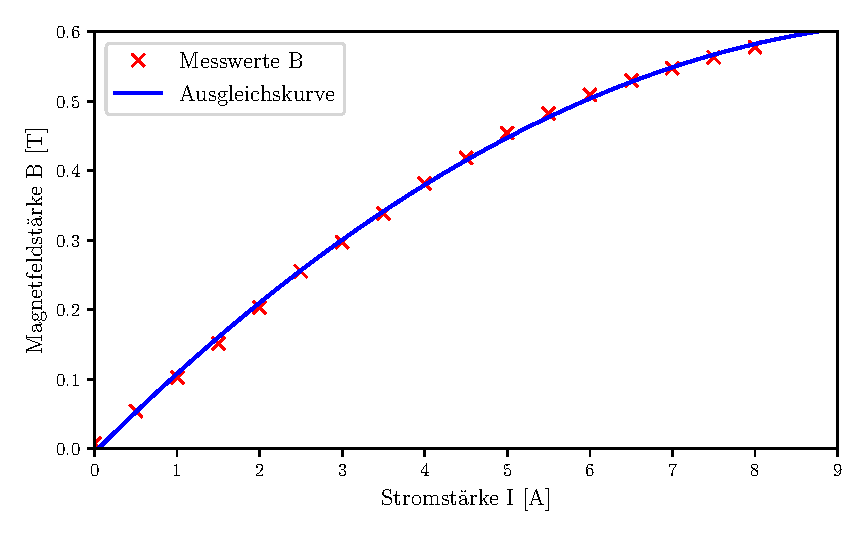
\includegraphics[scale=0.65]{Magnetfeld.pdf}
  \vspace{-10pt}
  \caption{Gemessenes Magnetfeld in Abhängigkeit von der Stromstärke.}
  \label{fig:Magnetfeld}
\end{figure}


\subsection{Rote Spektrallinie}
Abbildung \ref{fig:rot} zeigt die Spektrallinien der Wellenlänge $\lambda = 643,8$ nm. Dabei ist die obere Hälfte ohne Magnetfeld 
entstanden und die untere Hälfte mit Magnetfeld. Die Elektromagneten wurden mit $I = 8$ A betrieben, was aus Kapitel \ref{sec:Magnetfeld} 
einer Magnetfeldstärke von $B = 582,43 \pm 25.57$ mT entspricht.

\begin{figure}[H]
  \centering
  \includegraphics[width=\textwidth]{Rot.png}
  \vspace{-10pt}
  \caption{Interferenzmuster der Cd-Lampe für die rote Linie, mit und ohne Magnetfeld.}
  \label{fig:rot}
\end{figure}
Mit der Formel 

\begin{equation}
  \label{equ:Wellenlänge}
  \delta \lambda = \frac{1}{2} \frac{\delta s}{\Delta s} \cdot \lambda_D
\end{equation}
und den Werten aus Tabelle \ref{tab:Rot}, kann nun die Wellenlängenverschiebung berechnet werden.

\begin{table}
  \centering
  \footnotesize
  \caption{Abstände der Interferenzmaxima der roten Interferenzmuster.}
  \label{tab:Rot}

  \begin{tabular}{r r r}
    \toprule
    Ordnung & $\Delta s$ / px & $\delta s$ / px\\
    \midrule
    1   & 198 & 92  \\
    2   & 204 & 98  \\
    3   & 207 & 103 \\
    4   & 214 & 102 \\
    5   & 218 & 106 \\
    6   & 225 & 109 \\
    7   & 234 & 113 \\
    8   & 235 & 117 \\
    9   & 255 & 119 \\
    10  & 261 & 122 \\
    \bottomrule
  \end{tabular}
\end{table}

Zudem wird die Wellenlänge des Dispersionsgebiets $\lambda_D = 48,94$ pm benötigt.
Aus all diesen Werten ergibt sich eine Wellenlängenverschiebung von: \\
$\delta \lambda = 11,76 \pm 0,09$ pm

Mit dieser Wellenlänngenverschiebung kann der Lande-Faktor berechnet werden.
Dafür wird zunächst

\begin{equation}
  \label{equ:Lande}
  g_{ij} = m_1 g_1 - m_2 g_2 = \frac{\Delta E }{\mu_B B}
\end{equation}
aufgestellt.
Anschließend wird die Energiedifferenz durch 

\begin{equation}
  |\Delta E| \approx \left | \frac{\delta E}{\delta \lambda} \right | \cdot |\delta \lambda | = \frac{h c}{\lambda^2} \cdot \delta \lambda
\end{equation}
beschrieben und in Gleichung \eqref{equ:Lande} eingesetzt.
Daraus ergibt sich für den Lande-Faktor,

\begin{equation}
  g = \delta \lambda \frac{hc}{\mu_B B \lambda^2}.
\end{equation}
Somit ist der Lande-Faktor für die Rote Spektrallinie:\\
$g = 1,04 \pm 0,05$


\subsection{Blaue Spektrallinie}
Abbildung \ref{fig:BlauS} zeigt die Blaue Spektrallinie der Wellenlänge $\lambda = 480$ nm. 
Im oberen Bereich sind die Linien ohne Magnetfeld zu sehen und im unteren mit Magnetfeld. Durch den Polarisationsfilter sind lediglich die $\sigma$-Linien sichtbar.
An den Elektromagneten sind in dem Fall $I = 3,75$ A angeschlossen, was nach Kapitel \ref{sec:Magnetfeld} $B = 361,02 \pm 10,14$ mT sind.

\begin{figure}[H]
  \centering
  \includegraphics[width=\textwidth]{Blau_Sigma.png}
  \vspace{-10pt}
  \caption{Interferenzmuster der Cd-Lampe für die blaue $\sigma$-Linie, mit und ohne Magnetfeld.}
  \label{fig:BlauS}
\end{figure}
In Tabelle \ref{tab:BlauS} sind die Abstände der verschiedenen Maxima, des Interferenzmusters mit und ohne Manetfeld, aufgelistet.

\begin{table}
  \centering
  \footnotesize
  \caption{Abstände der Interferenzmaxima der Blauen Interferenzmuster.}
  \label{tab:BlauS}

  \begin{tabular}{r r r}
    \toprule
    Ordnung & $\Delta s$ / px & $\delta s$ / px\\
    \midrule
    1   & 152 & 72 \\
    2   & 156 & 74 \\
    3   & 158 & 82 \\
    4   & 156 & 80 \\
    5   & 162 & 84 \\
    6   & 158 & 78 \\
    7   & 154 & 80 \\
    8   & 160 & 82 \\
    9   & 168 & 78 \\
    10  & 156 & 86 \\
    \bottomrule
  \end{tabular}
\end{table}

Zusammen mit Gleichung \eqref{equ:Wellenlänge} und der Wellenlänge des Dispersionsgebiets für die blauen Spektrallinien $\lambda_D = 26,95$ pm ergibt sich 
daraus eine Wellenlängenverschiebung von: \\
$\delta \lambda = 6,79 \pm 0,11$ pm\\
Der Lande-Faktor wird mit Hilfe von Formel \eqref{equ:Lande} berechnet:\\
$g = 1,75 \pm 0,06$



